\documentclass[tikz,border=3.14mm]{standalone}
\usepackage{amsmath}

\begin{document}
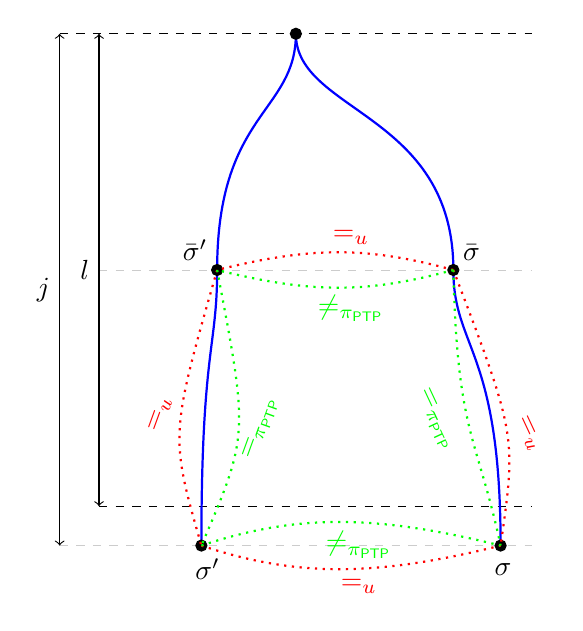
\begin{tikzpicture}
    % Define lengths
    \def\lc{3} % Length of lc
    \def\ls{3} % Length of ls

    % Draw horizontal dashed lines (was vertical in horizontal version)
    \draw[dashed] (-1,0) -- (5,0);
    \draw[dashed,ultra thin, opacity = 0.2] (-0.5,-\lc) -- (5,-\lc);
    \draw[dashed] (-0.5,-\lc-\ls) -- (5,-\lc-\ls);
    \draw[dashed, ultra thin, opacity = 0.2] (-1,-\lc-\ls-0.5) -- (5,-\lc-\ls-0.5);

    % Draw vertical lines for lc and ls (was horizontal in horizontal version)
    \draw[<->] (-0.5,0) -- (-0.5,-\lc-\ls) node[midway,left] {$l$};
    \draw[<->] (-1,0) -- (-1,-\lc-\ls-0.5) node[midway,left] {$j$};

    % Draw curves
    \draw[thick,blue] (2,0) .. controls (2,-\lc/3) and (4,-\lc/3) .. (4,-\lc)
        .. controls (4,-\lc-\ls/3) and (4.6,-\lc-\ls/3) .. (4.6,-\lc-\ls-0.5) node[below] {};

    \draw[thick,blue] (2,0) .. controls (2,-\lc/3) and (1,-\lc/3) .. (1,-\lc)
        .. controls (1,-\lc-\ls/3) and (0.8,-\lc-\ls/3) .. (0.8,-\lc-\ls-0.5) node[below] {};

    % Add points
    \filldraw (2,0) circle (2pt);
    \filldraw (4,-\lc) circle (2pt);
    \filldraw (1,-\lc) circle (2pt);
    \filldraw (4.6,-\lc-\ls-0.5 ) circle (2pt);
    \filldraw (0.8,-\lc-\ls-0.5) circle (2pt);

    % Add labels for points
    \node[above right] at (4,-\lc) {$\bar{\sigma}$};
    \node[above left] at (1,-\lc) {$\bar{\sigma}'$};

    % Add labels
    \node[right] at (4.4,-\lc-\ls-0.8) {$\sigma $};
    \node[right] at (0.6,-\lc-\ls-0.8) {$\sigma' $};

% Draw dashed parallel curves from \bar{\sigma} and \bar{\sigma'}
      
   

  

    % Draw red curve connecting \bar{\sigma} to \bar{\sigma'}
    \draw[red,dotted,thick] (4,-\lc) .. controls (2.9,-\lc+0.3) and (2.2,-\lc+0.3) .. (1,-\lc);

    \draw[green,dotted,thick] (4,-\lc) .. controls (2.9,-\lc-0.3) and (2.2,-\lc-0.3) .. (1,-\lc);


    \draw[red,dotted,thick] (1,-\lc) .. controls (0.4,-\lc-\ls+0.9) and (0.4,-\lc-\ls+0.9) .. (0.8,-\lc-\ls-0.5);

    \draw[green,dotted,thick] (1,-\lc) .. controls (1.4,-\lc-\ls+0.9) and (1.4,-\lc-\ls+0.9) .. (0.8,-\lc-\ls-0.5);
    
    

    % WORKING HERE NOW
    \draw[red,dotted,thick] (4,-\lc) .. controls (4.8,-\lc-\ls+0.9) and (4.8,-\lc-\ls+0.9) .. (4.6,-\lc-\ls-0.5 );

    \draw[green,dotted,thick] (4,-\lc) .. controls (4.05,-\lc-\ls+0.9) and (4.3,-\lc-\ls+0.9) .. (4.6,-\lc-\ls-0.5 );





    \draw[red,dotted,thick] (0.8,-\lc-\ls-0.5) .. controls (2,-\lc-\ls-0.9) and (3,-\lc-\ls-0.9) .. (4.6,-\lc-\ls-0.5);
    




    \draw[green,dotted,thick] (0.8,-\lc-\ls-0.5) .. controls (2,-\lc-\ls-0.1) and (3,-\lc-\ls-0.1) .. (4.6,-\lc-\ls-0.5);


    % Add label for the red curve

    
    \node[above] at (2.7,-\lc+0.2) {${\color{red}=_{u}}$};
    \node[below] at (2.7,-\lc-0.2) {${\color{green}\neq_{\pi_{\textsf{PTP}}}}$};

    \node[left, rotate=70] at (0.4,-\lc-\ls+1.5) {${\color{red}=_{u}}$};
    \node[left, rotate=70] at (1.74,-\lc-\ls+1.5) {${\color{green}=_{\pi_{\textsf{PTP}}}}$};
   \node[left, rotate=-65] at (5.1,-\lc-\ls+0.6) {${\color{red}=_{u}}$};
   \node[left, rotate=-65] at (4,-\lc-\ls+0.6) {${\color{green}=_{\pi_{\textsf{PTP}}}}$};

   \node[below] at (2.8,-\lc-\ls-0.2) {${\color{green}\neq_{\pi_{\textsf{PTP}}}}$};

   \node[below] at (2.8,-\lc-\ls-0.8) {${\color{red}=_{u}}$};
\end{tikzpicture}
\end{document}
